
\section{Introduction to Excel}

Microsoft Excel is the spreadsheet program we will use for much of our
data analysis and graphing.  It is a powerful and easy-to-use
application for graphing, fitting, and manipulating data. In this
appendix, we will briefly describe how to use Excel to do some useful
tasks.  The current version is Excel 2013.

\subsection{Data and formulae}

Figure \ref{fig:excel} below shows a sample Excel spreadsheet containing data
from a made-up experiment.  The experimenter was trying to measure
the density of a certain material by taking a set of cubes
made of the material and measuring their masses and the lengths of
the sides of the cubes.  The first two columns contain her measured
results.  \textbf{Note that the top of each column contains both
a description of the quantity contained in that column and its units.}
You should make sure that all of the columns of your data tables do as well.
You should also make sure that the whole spreadsheet has a descriptive
title and your names at the top, as indicated in the sample spreadsheet 
below.

\begin{figure}[b!]
\centerline{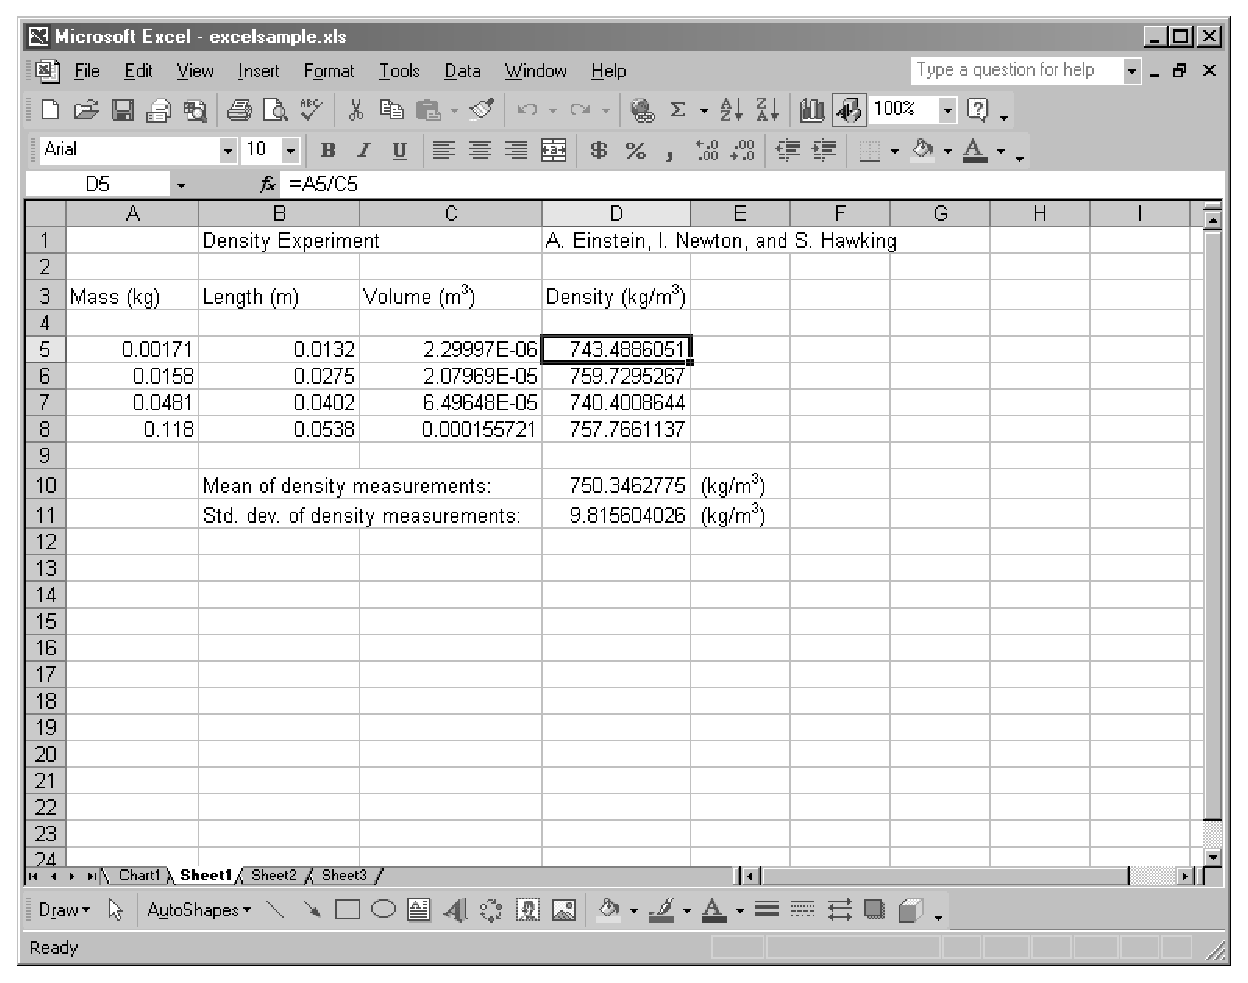
\includegraphics[width=3in]{../../131/StudentGuideModule1/appendices/excel/excelfigs/excelwindow.eps}}
\caption{Sample Excel spreadsheet}
\label{fig:excel}
\end{figure}

In the third column, the experimenter has figured out the volume
of each of the cubes, by taking the cube of the length of a side.
To avoid repetitious calculations, she had Excel do this automatically.
She entered the formula {\tt =B5$\wedge$3}  into cell C5.
Note the equals sign, which indicates to Excel that a formula is coming.
The $\wedge$ sign stands for raising to a power.  After entering a formula
into a cell, you can grab the square in the lower right corner of the
cell with the mouse and drag it down the column, or you can just double-click
on that square.  (Either way, note that thing you're clicking on is
the tiny square in the corner; clicking somewhere else in the cell won't work.)
This will copy
the cell, making the appropriate changes, into the rest of the column.
For instance, in this case, cell C6 contains the formula {\tt =B6$\wedge$3},
and so forth.

Column D was similarly produced with a formula that divides the
mass in column A by the volume in column C.

At the bottom of the spreadsheet we find the mean and standard
deviation of the calculated densities (that is, of the numbers
in cells D5 through D8).  Those are computed
using the formulae {\tt =average(D5:D8)} and {\tt =stdev(D5:D8)}.




\subsection{Graphs}

Here's how to make graphs in Excel.  First, use the mouse
to select the columns of numbers you want to graph.  (If the two
columns aren't next to each other, rearrange them so that they are next to 
each other. The variable you want on the horizontal axis needs to be to the 
left of the variable you want on the vertical axis).
Then click on the {\tt Insert} tab at the top of the window.
In the menu that shows up, there is a section called {\tt Charts}.
Almost all of the graphs we make will be scatter plots (meaning plots
with one point for each row of data), so click on the {\tt Scatter} icon, 
which is the lower one in the group that looks like this  

\includegraphics[width=0.2in]{../../131/StudentGuideModule1/appendices/excel/excelfigs/scatterplot.eps}.  
Several possible scatter plots appear. Select the 
first one with the same icon as before, and your graph will appear.
\vspace{0.5cm}

Next, you'll need to customize the graph in various ways, such
as labeling the axes correctly.  
%Everything you need to do this is in the {\tt Chart Tools} menu, which should
%be visible in the upper right portion of the window.  (If you
%don't see the words {\tt Chart Tools}, try clicking on your newly-created
%graph, and it should appear.)  The most useful items are under
%the {\tt Layout} tab, so click on the word {\tt Layout} under the {\tt Chart
%Tools} menu.  Here are some things to do under this menu:
\vspace{0.5cm}

This is done in the {\tt Chart Elements} menu which is accessed by clicking 
on the plus sign (+) in a box, at the upper right corner of your graph. Click 
on {\tt Axis Titles}, and places appear for axis titles. Edit the text inside 
of the two axis titles so that it indicates what's on the two axes of your 
graph, {\it including the appropriate units for each}.
\vspace{0.5cm}

Next, give your graph an overall title. Click on {\tt Chart Title} and a box 
appears around it. Delete ``Chart Title'' and enter a proper title such as 
``Position vs Time'' or whatever.
\vspace{0.5cm}

Usually you want your graph to contain a best-fit line passing
through your data points.  To do this, right click on one of the data points 
and select {\tt Add Trendline}. A number of options appear such as 
``linear'', ``polynomial'', ``power'', and so on.  Select the one you want, 
and also check the {\tt Display Equation on chart} option near the bottom. 
You can then drag the equation to someplace else on the chart so you can read 
it better. Remember that Excel won't include the correct units on the numbers 
in this equation, but you should.  Also, Excel will always call the two 
variables $x$ and $y$, even though they might be something else entirely. Bear 
these points in mind when transcribing the equation into your lab notebook.
\vspace{0.5cm}



Sometimes, you may want to make a graph in Excel where the $x$ column
is to the right of the $y$ column in your worksheet.  In these cases,
Excel will make the graph with the $x$ and $y$ axes reversed. Here's how 
to fix this problem:  Before you make your graph,  make a copy of the $y$ 
column in the worksheet and paste it so that it's to the right of the $x$ 
column.  Then follow the above procedure and everything will be fine.
%If you don't want to do that, here's
%another way.  Click {\tt Select data} (near the left-hand side under
%the Chart Tools menu).  In the box that pops up, highlight {\tt Series1}
%and click {\tt Edit}.  You should see a box that contains entries
%for {\tt Series X values} and {\tt Series Y values}.  You want to swap the 
%entries in those two windows.  (But really, it's much easier
%to do it the first way.)


\subsection{Making Histograms}

A histogram is a useful graphing tool when you want to analyze groups of data, based on the frequency at given intervals. 
In other words, you graph groups of numbers according to how often they appear.
You start by choosing a set of `bins', {\it i.e.}, creating a table of numbers that mark the edges of the intervals.
You then go through your data, sorting the numbers into each bin or interval, and tabulating the number of data points that fall into each bin (this is the 
frequency).
At the end, you have a visualization of the distribution of your data.   

Start by entering your raw data in a column like the one shown in the left-hand panel of Figure \ref{hist2}.
\begin{figure}[b!]
\begin{center}
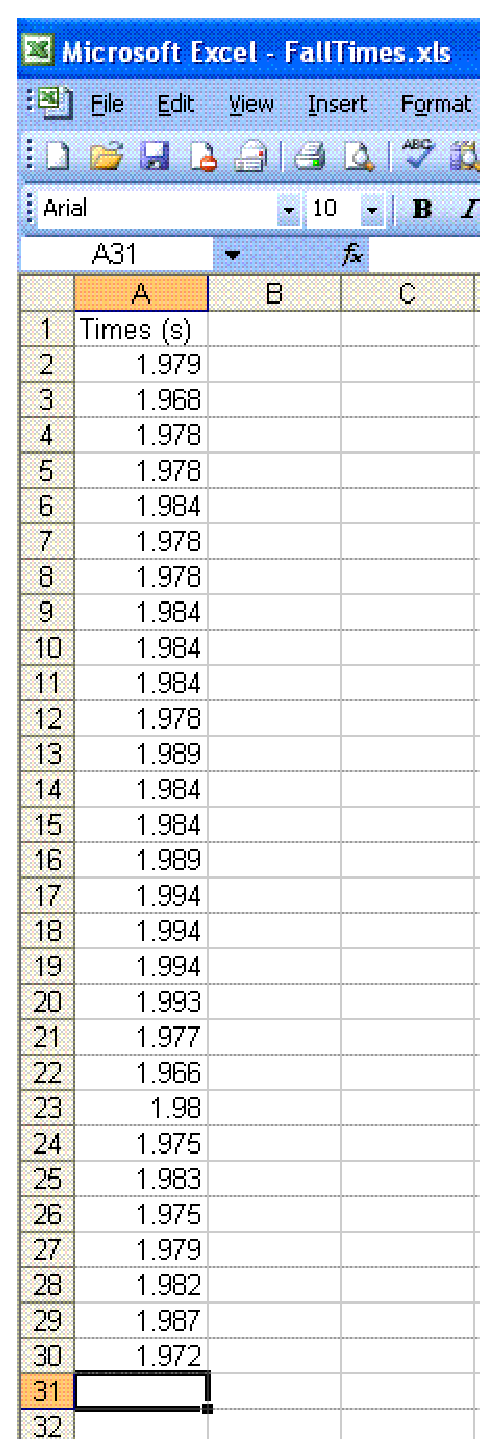
\includegraphics[height=2.5in]{../../131/StudentGuideModule1/appendices/excel/excelfigs/histf1.eps}
\hspace{0.4in}
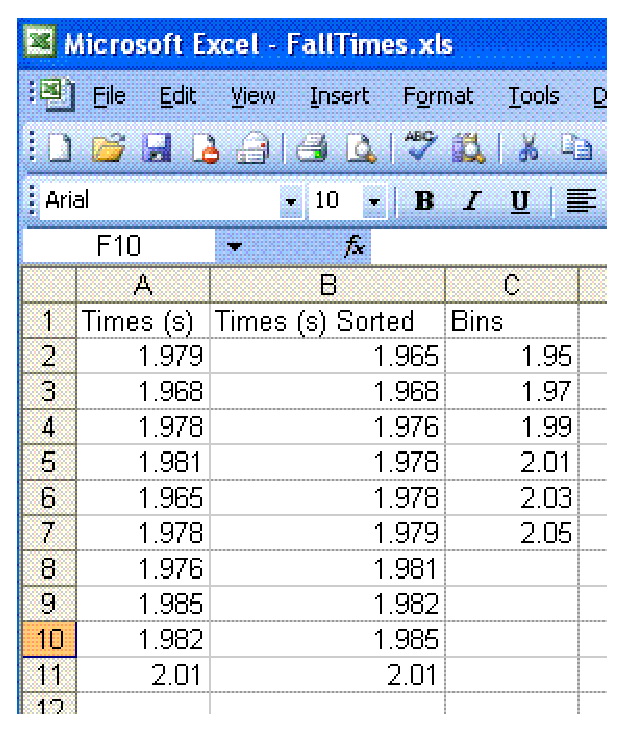
\includegraphics[height=2.5in]{../../131/StudentGuideModule1/appendices/excel/excelfigs/histf2.eps}
\caption{Column data and bins (left-hand panel) and dialog box (right-hand panel)  for making a histogram in Excel.}\label{hist2}
\end{center}
\end{figure}
Look over your numbers to see what is the range of the data.
If you have lots of values to sift through you might consider sorting your data is ascending or descending order.
(You don't need to do this if you can easily see the range of data.)
To do this task, choose the column containing your data by clicking on the letter at the top of the column, 
go to {\tt Data} in the menubar, select {\tt Sort}, and pick
ascending or descending.
The data will be rearranged in the order you've chosen and it will be easier to see the range of the data.
For an example, see the middle column of data in the left-hand panel of Figure \ref{hist2}.


Now to create your bins pick a new column on your spreadsheet and enter the values of the bin edges.
Bins should be of equal size with the bin edges given by simple numbers.
Make sure the bins you choose cover the range of the data. 
See the left-hand panel of Figure \ref{hist2} again for an example.

\newpage

You now have the ingredients for making the histogram.
Go to {\tt Data} in the menubar, select {\tt Data Analysis} (on the right) and 
choose {\tt Histogram}. Click {\tt OK}.
You should see a dialog box like the one in the right-hand panel of  Figure \ref{hist2}.
Click in the box labeled {\tt Input Range} and then highlight the column on the spreadsheet containing your data.
Next, click in the box labeled {\tt Bin Range} and highlight the column on the spreadsheet containing the bins.
Under {\tt Output Options}, select {\tt Chart Output} and click {\tt OK}. The histogram should come up. 
If it doesn't, go to {\tt Insert} in the menubar and select 
the histogram icon in the {\tt Charts} section (the first icon in that section).
Change the horizontal axis label to whatever you are plotting (including units). The vertical axis should already be labeled "Frequency".
Change the chart title to an appropriate title for whatever you are plotting. 
The result should look like the right hand panel of Figure \ref{hist5}.
%Click {\tt OK} in the {\tt Histogram} dialog box.
%You should now see a new worksheet with columns labeled {\tt Bin} and {\tt Frequency} and a new tab at the bottom with the name you put in
%the {\tt New Worksheet Ply} entry.
%See the left-hand panel in Figure \ref{hist5}.
\begin{figure}[b!]
\begin{center}
\includegraphics[height=2.5in]{../../131/StudentGuideModule1/appendices/excel/excelfigs/histf3.eps}
\hspace{0.4in}
\includegraphics[height=2.5in]{../../131/StudentGuideModule1/appendices/excel/excelfigs/histf4.eps}
\caption{Newly-created worksheet (left-hand panel) and final plot (right-hand panel) for  histogram worksheet in Excel.}\label{hist5}
\end{center}
\end{figure}
%Your original data are still available on another worksheet (probably labeled {\tt Sheet1}).
%Now highlight the {\tt Bins} and {\tt Frequency} columns by clicking and dragging across the column headings (the {\tt A} and {\tt B}
%at the top of the columns in the left-hand panel of Fig. \ref{hist5}).
%You can then make a graph by following the procedure in Appendix C.2 above.
%The only difference is that this time you will choose to make a {\tt Column}
%graph instead of a {\tt Scatter} graph.
%Make sure you properly label the axes including the units for each quantity.
%Results should look like the right-hand panel of Figure \ref{hist5}.

\newpage

\subsection{LINEST}

LINEST is a function in Excel which gives a LINear ESTimate of the slope and the uncertainty in the slope for any linear data set. The uncertainty is based on the scatter of the data points about a perfect straight line. To use LINEST in Excel, perform the following steps:

\begin{enumerate}

\item Select a 2 x 2 group of cells (not including any cells with data)
\item In the function line type =LINEST(
\item Select range of $y$ values
\item Type comma (,)
\item Select range of $x$ values
\item Type comma (,)
\item Type 1,1)
\item Hold down control AND shift buttons, press enter
\item The result should look like this:

\begin{center} \begin{tabular}{|c|c|} \hline slope & intercept \\ \hline \( \Delta \)slope & \( \Delta \)intercept \\ \hline \end{tabular} \end{center}

\end{enumerate}

\( \Delta \)slope represents the uncertainty in the slope value. You will still need to round off both numbers, depending on the relative magnitudes of the two numbers. It is also common practice to express both numbers to the same power of 10.

